%\section{Physical Human Factors Report: Tristan Griffith}
\rhead{\today}
\begin{center}
{\textbf{\Large Brief on Modal EEG Fingerprinting}}\\
\vspace{2mm}
{\large  Tristan Griffith}\\
\vspace{2mm}
{\large Dr. James Hubbard Jr.}
\noindent\rule{\textwidth}{2pt}
\end{center}

%\begin{wrapfigure}{r}{0.45\textwidth}
%\centering
%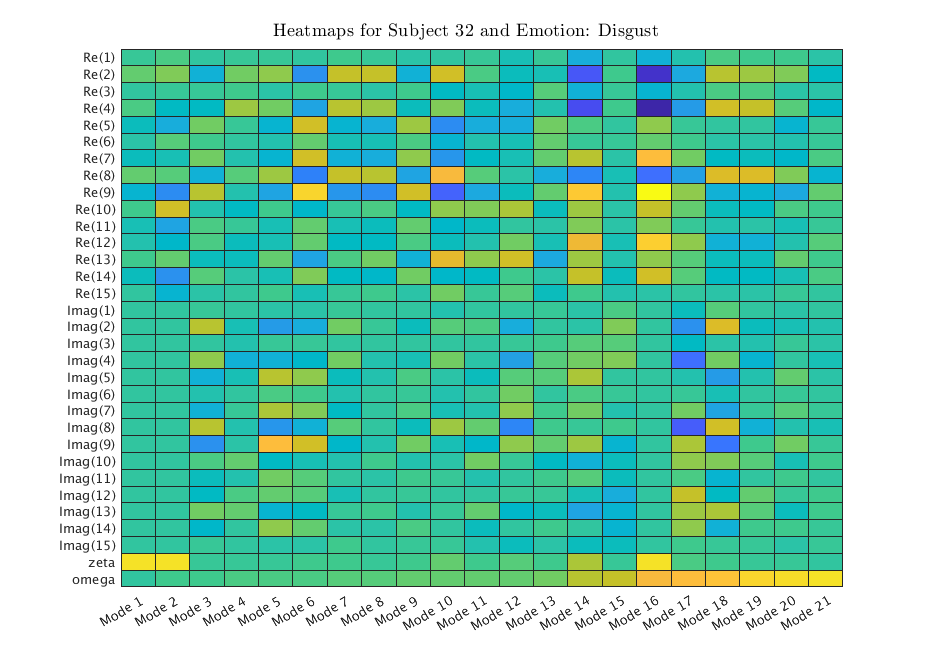
\includegraphics[scale=.3]{../../../figures/demo_map.png} 
%\caption{Modal Heatmap for Subject 32}
%\end{wrapfigure}
\subsection{Motivation}
A correlation between electrical activity in the brain (as electroencephalography) and cognition has already been established \cite{alarcao2017emotions}. However, formal models of this relationship have thus far been experimentally limited. We postulate that data driven system identification methods of EEG data, such as Output Only Modal Analysis and Dynamic Mode Decomposition, may yield predictive models of cognition for more complete information flow between human operators and co-robots. As an initial step to verify that there is statistically significant information in these modal representations, an artificial neural network is proposed to discriminate subjects in a database. If the network shows sufficient accuracy in identifying subjects from the modal representation of their brain activity, we gain confidence that the modal representation is capturing significant information in the modes. This document surveys this approach and details the results of the network. It is shown that the network can discriminate 32 subjects from one another with $<99$\% accuracy based on knowledge of the significant modes alone.
\subsection{The EEG Dataset}
The data used to test this modal decomposition approach is primarily the DEAP dataset \cite{koelstra2011deap}. This dataset was established to aid the analysis of human affective states. It includes 40 different minute long  trials for 32 different subjects. From this timeseries EEG data with 32 available spatial channels, 1280 modal decompositions will be performed. 1024 of these decompositions are provided to the neural network for training, while the remaining 256 decompositons will be used to validate the performance of the network. A closer look at the modal decomposition follows.
\subsection{Modal Decomposition of Data}
\subsubsection{Output Only Modal Analysis (OMA)}
Output Only Modal Analysis (OMA) algorithms have been in use since at least the 90's \cite{peeters1999reference}. Originally developed for large mechanical structures, which are extremely difficult to precisely excite, OMA algorithms assume broadband stochastic input to the system in order to determine a state space model for a given system. These algorithms fall under a broader class of subspace identification methods, which rely directly on measured data. The specific method applied to this data results from solving a set of linear equations with least squares to match data held in a Hankel matrix \cite{261604}. Empirically, we have seen this algorithm perform more consistently on the DEAP dataset. That is, there is less variance in the generated modes for a given subject. 

%% ADD PLOT OF CLASSIFICATION ACC VS NUMBER OF CHANNELS, ALSO SYSTEM ORDER
To perform the modal decomposition presented below, the first 16 channels out of 32 available were selected for analysis. These 16 channels correspond to the electrodes placed on the front half of the scalp. The selection was driven by computational limits and the desire to use as few channels as possible for subject identification. Selection of the appropriate system order is also important. This is generally determined from the stability diagram, which gives insight into how much the 
\begin{wrapfigure}{r}{0.55\textwidth}
\centering
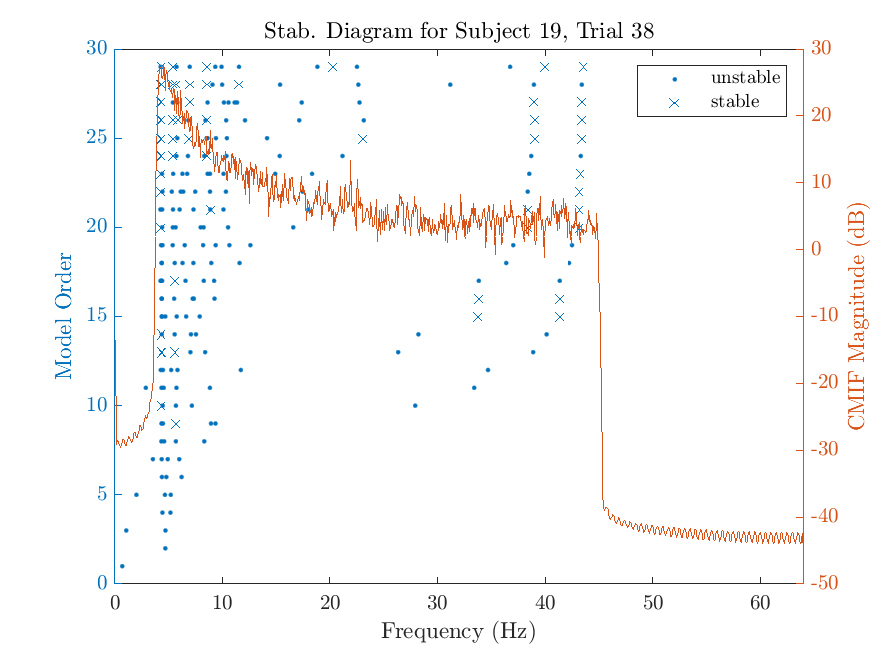
\includegraphics[scale=0.6]{../../../figures/S19T38.png}  
\caption{Stability Diagram for DEAP}
\label{fig:stabdiag}
\end{wrapfigure}
poles and zeros are changing as the model order increases. That is, we can track the percent change in the norm of the poles and zeros as additional states are added to the system. From Figure \ref{fig:stabdiag}, it can be seen that the system properties are more unstable than is typical for mechanical structures, especially at the higher frequencies. For the purposes of this brief, the selected subject order was 25, in order to capture the faster modes near the 45 hertz range. With these selections, 20 linearly independent, but not orthogonal modes are identified, ranging in frequency from 3-45 hertz. We postulate that these eigenvectors are relevant to emergent cognitive behaviors, such as engagement.   


\subsubsection{Dynamic Mode Decomposition (DMD)}
While OMA algorithms are considered subspace identification algorithms, there are other modal decomposition tools available. These include independent component analysis, principle component analysis, and proper orthogonal decomposition. An extension of proper orthogonal decomposition (POD) known as dynamic mode decomposition (DMD) has gained traction as data driven dynamic modeling and control becomes of increasing interest to the research community. DMD is based on the singular value decomposition, combining the spatial analysis of POD with the temporal analysis of the Fourier transform to estimate a state matrix directly from measured data. Unlike OMA algorithms, it makes no assumptions on the nature of the input. It has shown wide application in modeling of fluids dynamics \cite{schmid2010dynamic}, biological systems \cite{brunton2016extracting}, and human diseases \cite{proctor2015discovering}. 

Since DMD is a singular value method, generated modes are sorted by their importance in explaining the variance in the data. Once an acceptably accurate number of modes is selected, the state matrix may be truncated to that number of modes. Previous work has found selecting too many modes leads to decreased classification performance, due to the introduction of spurious modes as a form of noise \cite{jung1997estimating}.

\begin{figure}
\centering
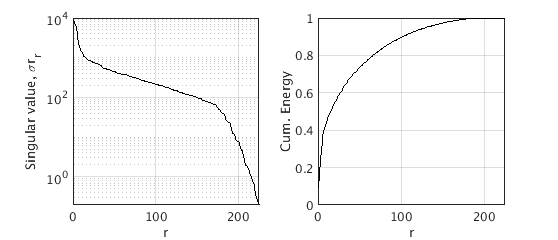
\includegraphics[scale=0.85]{../../../figures/S_r.png}
\caption{Significant Singular Values for DMD}
\label{fig:svd}
\end{figure}

For this data, approximately 80 modes were selected, describing $\approx 85$\% of the total energy in the system. This can be seen in Figure \ref{fig:svd} below. Keep in mind that as with OMA algorithms, DMD will generate complex conjugate mode pairs, so only 40 independent mode shapes of interest are actually identified. 

\subsection{Modal Decomposition as a Heatmap}
Having generated both OMA and DMD modes for 32 subjects over 40 trials in this data set, it is worth validating the quality of information in the modes. As a first check, we postulate that each of the 32 subjects may be distinguished from one another based solely on the significant modes. If a classification technique shows sufficient accuracy distinguishing subjects, we gain confidence that the modes contain statistically significant information.

\begin{wrapfigure}{r}{0.6\textwidth}
\centering
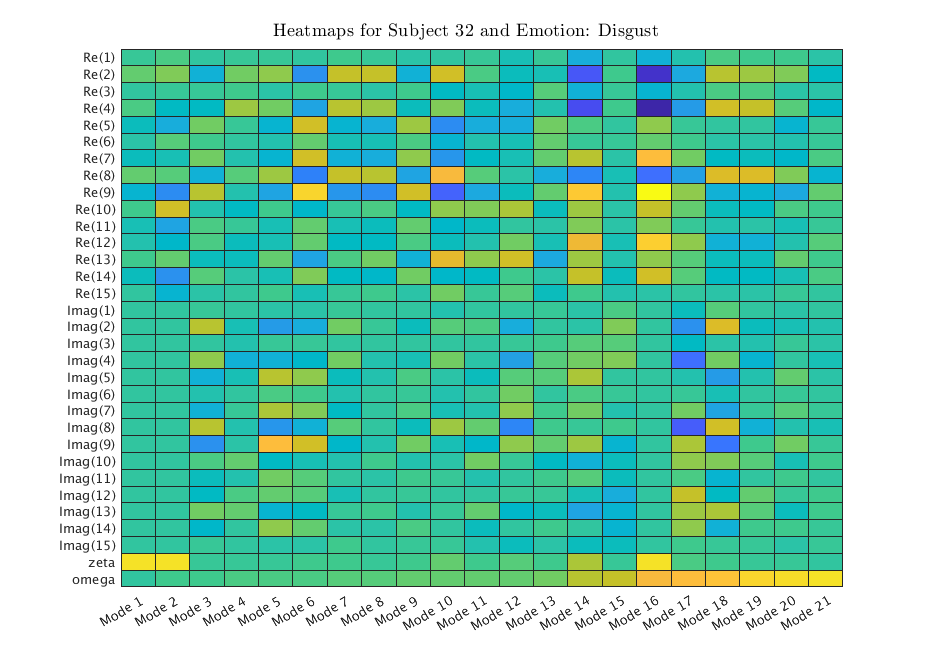
\includegraphics[scale=0.45]{../../../figures/demo_map.png} 
\caption{Modal Information Encoded as an Image}
\label{fig:heatmaps}
\end{wrapfigure}
The most obvious technique for this EEG fingerprinting classification is neural networks. Properly encoding these networks for efficient classification is important. While networks will readily accept modal information in a tabular form, recent advancements in gradient decent methods, transfer learning, etc are especially geared for three channel images. It is therefore desirable to transform our modal information into an RGB image. Image encoding of temporal and spatial information has seen wide application of late, with good success \cite{ke2020intersected, venugopal2020unboxing, bruno2019using}. The most obvious solution is to encode modal information as a heatmap with a color scale. Since both DMD and OMA algorithms allow for complex (out of phase) mode components, it is necessary to include both real and complex components as part of the image. This may be included as either a real and complex component or in polar form as an angle and amplitude. Along the x-axis of the figure is each of the modes, increasing in temporal frequency. Along the y-axis of the figure is the real or imaginary component of each spatial location of the given mode. This forms an image that is well suited for neural network classification. The authors wish to note that the application of machine learning in this case is used only as a validation technique for the modeling. The network is not used to discover the underlying dynamics of the system. Here, they merely serve as a check on the system identification techniques presented above.

\subsection{Neural Nets for Fingerprinting}
Having encoded our modal decompositions as images, the images may be fed to a neural network. Since it's inception in 2016, the ResNet architecture has served as a default method for computer vision machine learning due \cite{he2016deep}. It is important for this study to limit the complexity of the network as a further check on the validity of the data in the modal heatmaps. For this reason, an 18 layer ResNet architecture was selected for the subject classification model. That is, the network includes 18 linear transforms with a non-linearity in between each. For reference, default modern configurations of this architecture range from 18 to 152 layers. With 1024 heatmaps in the training set, and the remaining 256 reserved for validation, the network trains in fewer than 10 minutes total. The classification accuracy on unseen data is 98\% for the OMA modes, and 100\% for the DMD modes. The relevant confusion matrices are included in Figures \ref{fig:OMA} and \ref{fig:DMD}.
\begin{figure}[h!]
    \centering
    \begin{minipage}{0.45\textwidth}
        \centering
        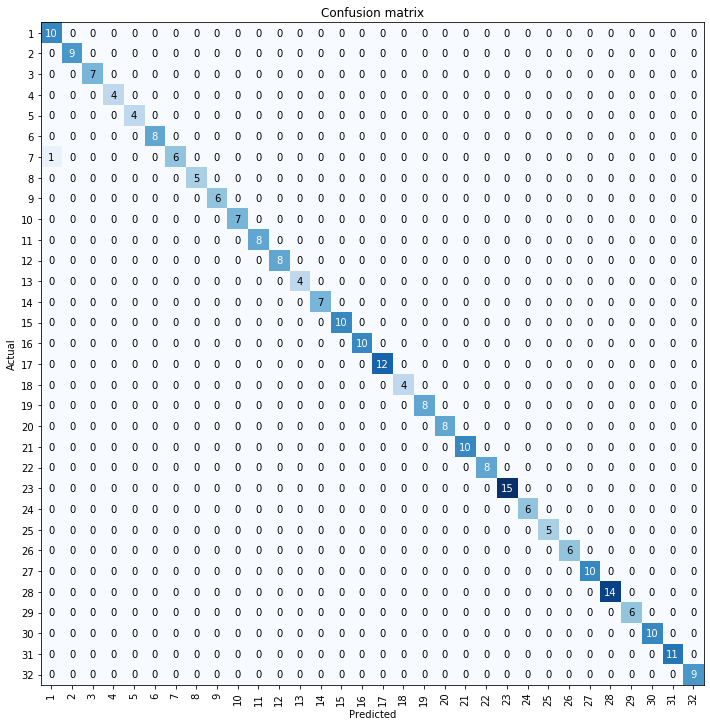
\includegraphics[scale=0.32]{../../../figures/conf_mat_OMA.png} % first figure itself
        \caption{Conf. Matrix for OMA Modes}
        \label{fig:OMA}
    \end{minipage}\hfill
    \begin{minipage}{0.45\textwidth}
        \centering
        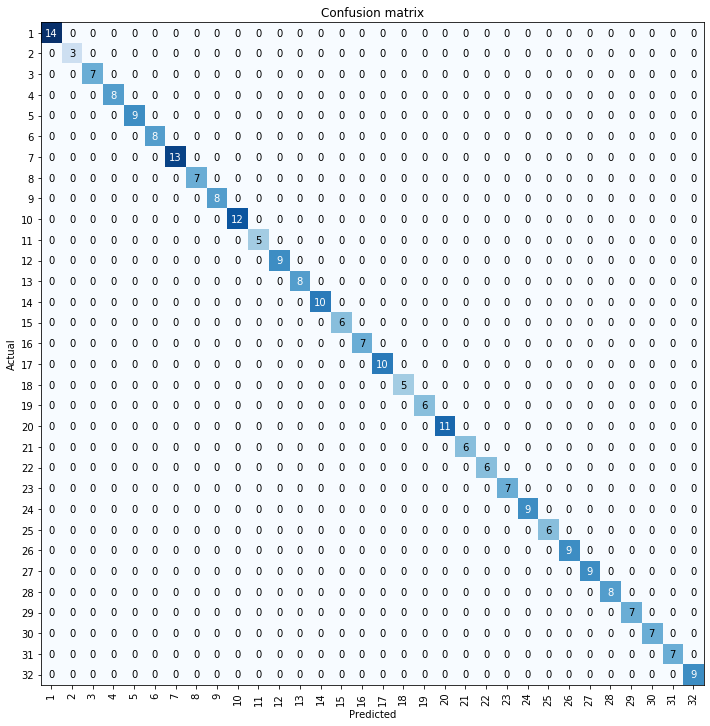
\includegraphics[scale=0.32]{../../../figures/conf_mat_DMD.png} % second figure itself
        \caption{Conf. Matrix for DMD Modes}
        \label{fig:DMD}
    \end{minipage}
\end{figure}

\subsection{Discussion}
These classification results are promising. On the Bayesian nature of neural networks alone, validation results approaching 100\% are very encouraging, especially with such a simple hypothesis class. The results also confirm existing knowledge that EEG data is interpersonally dependent \cite{makeig2012evolving}. This gives some initial credence to our system identification and modal approach to cognition. As a final check, we may ask how the network would perform if the labels were shuffled. The best we should expect this network to perform is 3.125\% accuracy ($1/32$), which is the best case scenario for a totally random guess, which represents the best case hypothesis for random subject labels. If, however, the network performs better, say any higher than 8\%, it may indicate that random noise can be permuted to match the labels we provided, even if they are not random.   
\begin{wrapfigure}{r}{0.6\textwidth}
\centering
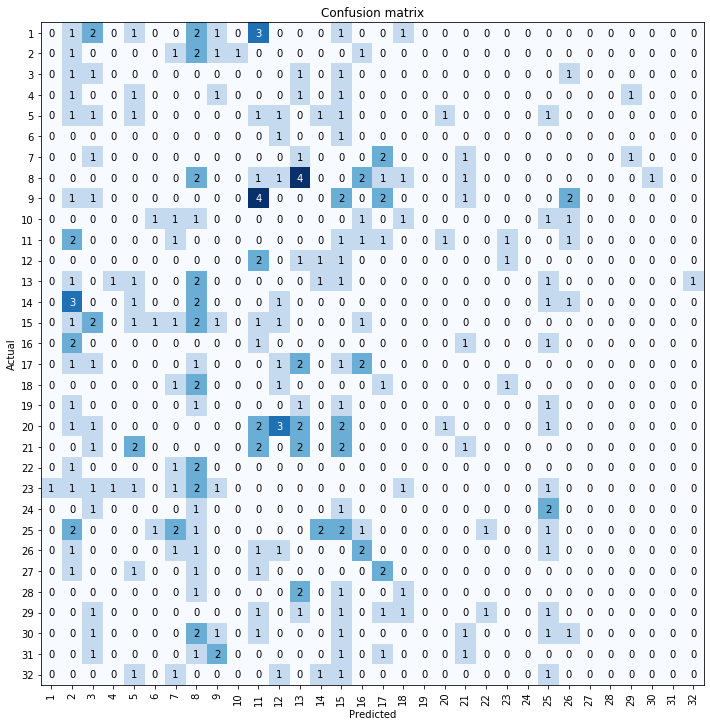
\includegraphics[scale=0.45]{../../../figures/conf_mat_random.png} 
\caption{Conf. Mat for Random Labels}
\label{fig:random}
\end{wrapfigure}  
Fortunately, in this case, the random label network shows approximately 3\% accuracy on unseen data. The relevant confusion matrix is included. This further increases our confidence on the modal decomposition. There is relevant information in the modes, and it can be used to identify one subject from another.

\begin{figure}[b]
    \centering
    \begin{minipage}{0.45\textwidth}
        \centering
        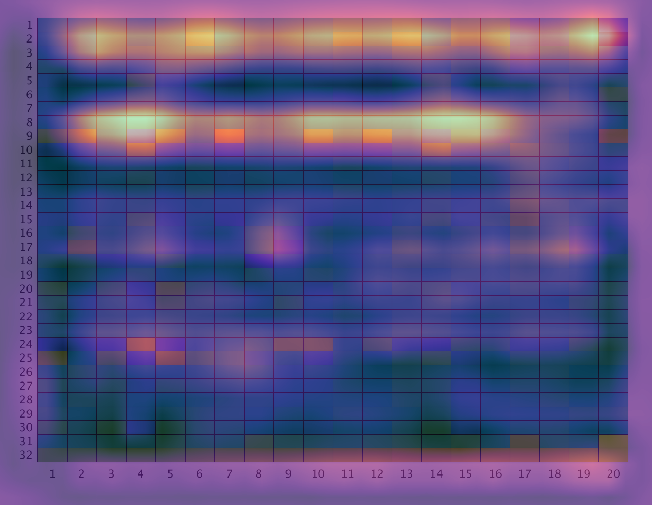
\includegraphics[scale=0.32]{../../../figures/heatmap_162_OMA.png} % first figure itself
        \caption{Focal Map for OMA Modes}
        \label{fig:OMA_heat}
    \end{minipage}\hfill
    \begin{minipage}{0.45\textwidth}
        \centering
        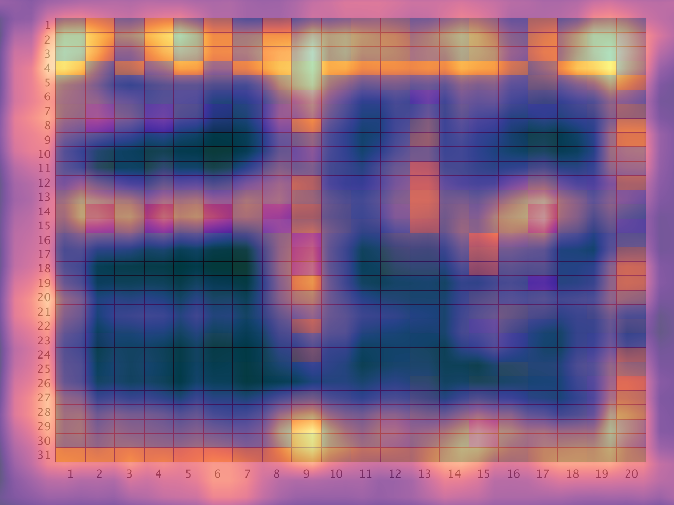
\includegraphics[scale=0.32]{../../../figures/heatmap_4_DMD.png} % second figure itself
        \caption{Focal Map for DMD Modes}
        \label{fig:DMD_heat}
    \end{minipage}
\end{figure}
From here, interpretation of the network results becomes relevant. Is the network relying on specific modes for classification? Is the real component more important than the complex component? Are the faster modes more important than the slow ones? Since neural networks are a gradient method, they assign a weight to each pixel in the image. We can track these weights and overlay them on the original image. Hot spots indicate special attention was paid by the network to make a classification, while cold spots indicate the opposite. Interestingly, the OMA and DMD representations drive the network to select different features for classification, while both show excellent results. The OMA network greatly relies on very few real components of all the modes. This corresponds to a single sensor location on the EEG device, suggesting interpersonal differences are highly constrained to spatial location. On the other hand, the DMD network seems to rely on specific modes, such as mode 9 in Figure \ref{fig:DMD_heat}. The additional noise surrounding the DMD network results in this figure may be a result of the data driven nature of the algorithm. In both cases, notice that neither network has any interest in the lower third of the image, which corresponds to the imaginary component of the modes.

\begin{wrapfigure}{r}{0.\textwidth}
\centering
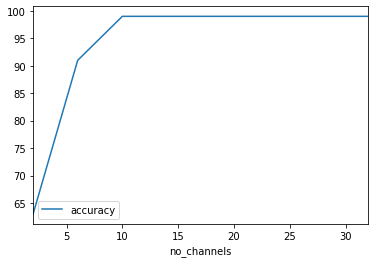
\includegraphics[scale=0.55]{../../../figures/channels.png} 
\caption{No. of Channels vs. Classification Accuracy}
\label{fig:channels}
\end{wrapfigure} 
Since the results seem highly dependent on just a few features, we may further ask if spatial sampling may be decreased. How few channels are necessary for accuracy classification results? Figure \ref{fig:channels} indicates that the minimum number of channels is somewhere between 5 and 10 for subject fingerprinting.

From these results, we now must think about connecting the modes to relevant emergent cognitive properties such as engagement. Perhaps we may remove the features that are used to identify subjects, resulting in a broadly applicable model of engagement. This portion of the work is ongoing, but encouraged by the success of the fingerprinting networks.
 






%\begin{displayquote}
%The class of monotone DNF expressions is learnable via an algorithm $B$ that uses $L=L(h,d)$ calls of examples and $dt$ calls of oracle, where $d$ is the degree of the DNF expression $f$ to be learnt and $t$ the number of variables.
%\end{displayquote}


%\begin{wrapfigure}{r}{0.55\textwidth}
%\centering
%\includegraphics[scale=.5]{../figures/complexity.png} 
%\caption{The Error-Complexity Trade Off}
%\end{wrapfigure}

